\begin{frame}{Agenda}
\begin{itemize}
    \item Introduction
    \item Literature Review
    \item \textbf{Methodology}
    \item Results
    \item Conclusion and Future Work
\end{itemize}
\end{frame}

%%

\begin{frame}{Methodology}
\begin{itemize}
    \item{On Target and Benchmark\\ }
        \begin{itemize}
            \item<2-> Terminology
            \item<2-> Block Diagram 
        \end{itemize}
    \vspace{0.3cm}
    \item{Clustering procedures\\}
        \begin{itemize}
            \item<3-> Strategy and Pairing 
            \item<3-> Number of Clusters
            \item<3-> Algorithm
        \end{itemize}
    \item{Experiments\\}
\end{itemize}
\end{frame}

%%

\begin{frame}{On Target and Benchmark - Terminology} 
    \pause
    \begin{itemize}
        \item Portfolio
        \vspace{0.1cm}
        \item Market
        \vspace{0.1cm}
        \item Features
        \vspace{0.1cm}
        \item Study
        \vspace{0.1cm}
        \item Experiment
    \end{itemize}
\end{frame}

%%

\begin{frame}{On Target and Benchmark - Diagrams}
    \imagem{fig/ch3-ot-blocks.png}{fig:ot-blocks}{Block Diagram of the On Target.}
\end{frame}

%%

\begin{frame}{On Target and Benchmark - Diagrams} 
    \imagem{fig/ch3-ot-benchmark-blocks.png}{fig:ot-benchmark-bloks}{Modifications on the OT done by the Benchmark.}
\end{frame}

%%

\begin{frame}{Clustering - Strategy and Pairing} \pause
    Two clustering strategies\\ \pause 
    \begin{itemize}
        \item \fullNameClusterStrategyA{} (\nameClusterStrategyA{})
        \item \fullNameClusterStrategyB{} (\nameClusterStrategyB{})
    \end{itemize}
\end{frame}

%%

\begin{frame}{Clustering - Strategy}
    \begin{figure}
        \centering
        \caption{Example of "\fullNameClusterStrategyA{}".}
        \begin{subfigure}{0.45\textwidth}
            \centering
            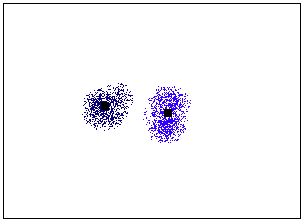
\includegraphics[width=\linewidth]{fig/ch3-cluster-strategy-port-fit.png}
            \caption{KMeans learning the centroids from portfolio data.}
            \label{fig:sub1}
        \end{subfigure}\hskip 1em \pause
        \begin{subfigure}{0.45\textwidth}
            \centering
            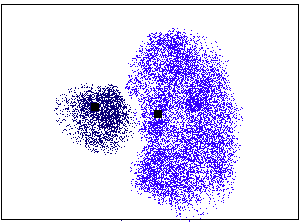
\includegraphics[width=\linewidth]{fig/ch3-cluster-strategy-port-predict.png}
            \caption{KMeans "prediction" to all data, with centroids learned from (\subref{fig:sub1}).}
            \label{fig:sub2}
        \end{subfigure}
    \end{figure}
\end{frame}

%%

\begin{frame}{Clustering - Strategy}
    \begin{figure}
        \centering
        \caption{Example of \fullNameClusterStrategyB{}}
        \begin{subfigure}{\textwidth}
            \centering
            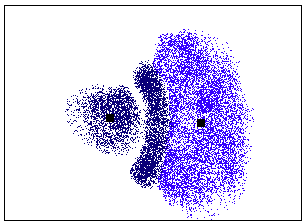
\includegraphics[width=0.5\linewidth]{fig/ch3-cluster-strategy-all.png}
            \caption{KMeans learning and "predicting" to all data.}
            \label{fig:sub3}
        \end{subfigure}
    \end{figure}
\end{frame}

%%

\begin{frame}{Clustering - Strategy and Pairing} \pause
    Two ways to pair the clusters\\ \pause
    \begin{itemize}
        \item \fullNameClusterPairingA{} (\nameClusterPairingA{})
        \item \fullNameClusterPairingB{} (\nameClusterPairingB{})
    \end{itemize}
\end{frame}

%%

\begin{frame}{Clustering - Pairing}
    \begin{figure}
        \centering
        \caption{
        Top: "\fullNameClusterPairingA{}" (\nameClusterStrategyA{}) \\
        Bottom: "\fullNameClusterPairingB{}" (\nameClusterStrategyB{}).}       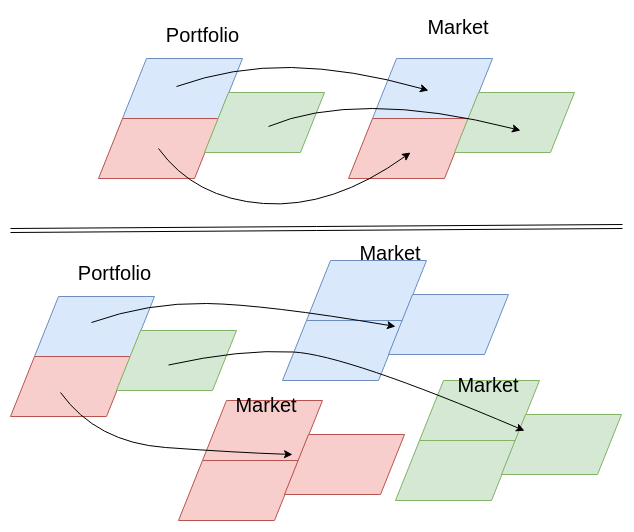
\includegraphics[height=6cm]{fig/ch3-cluster-pairing.png}
        \label{fig:cluster-pairing}
    \end{figure}
\end{frame}

%%

\begin{frame}{Clustering - Number of Clusters} \pause
    Manually \\  \pause
    \vspace{0.5cm}
    PCA Plot \\ \pause
    \vspace{0.5cm}
    Transformations \\ \pause
        \begin{itemize}
            \item One Hot Encoding (categorical) \pause
            \item Z-score Normalization 
        \end{itemize}
\end{frame}

%%

\begin{frame}{Clustering - Number of Clusters}
    \begin{figure}
        \centering
        \caption{PCA Plot for all features.} 
        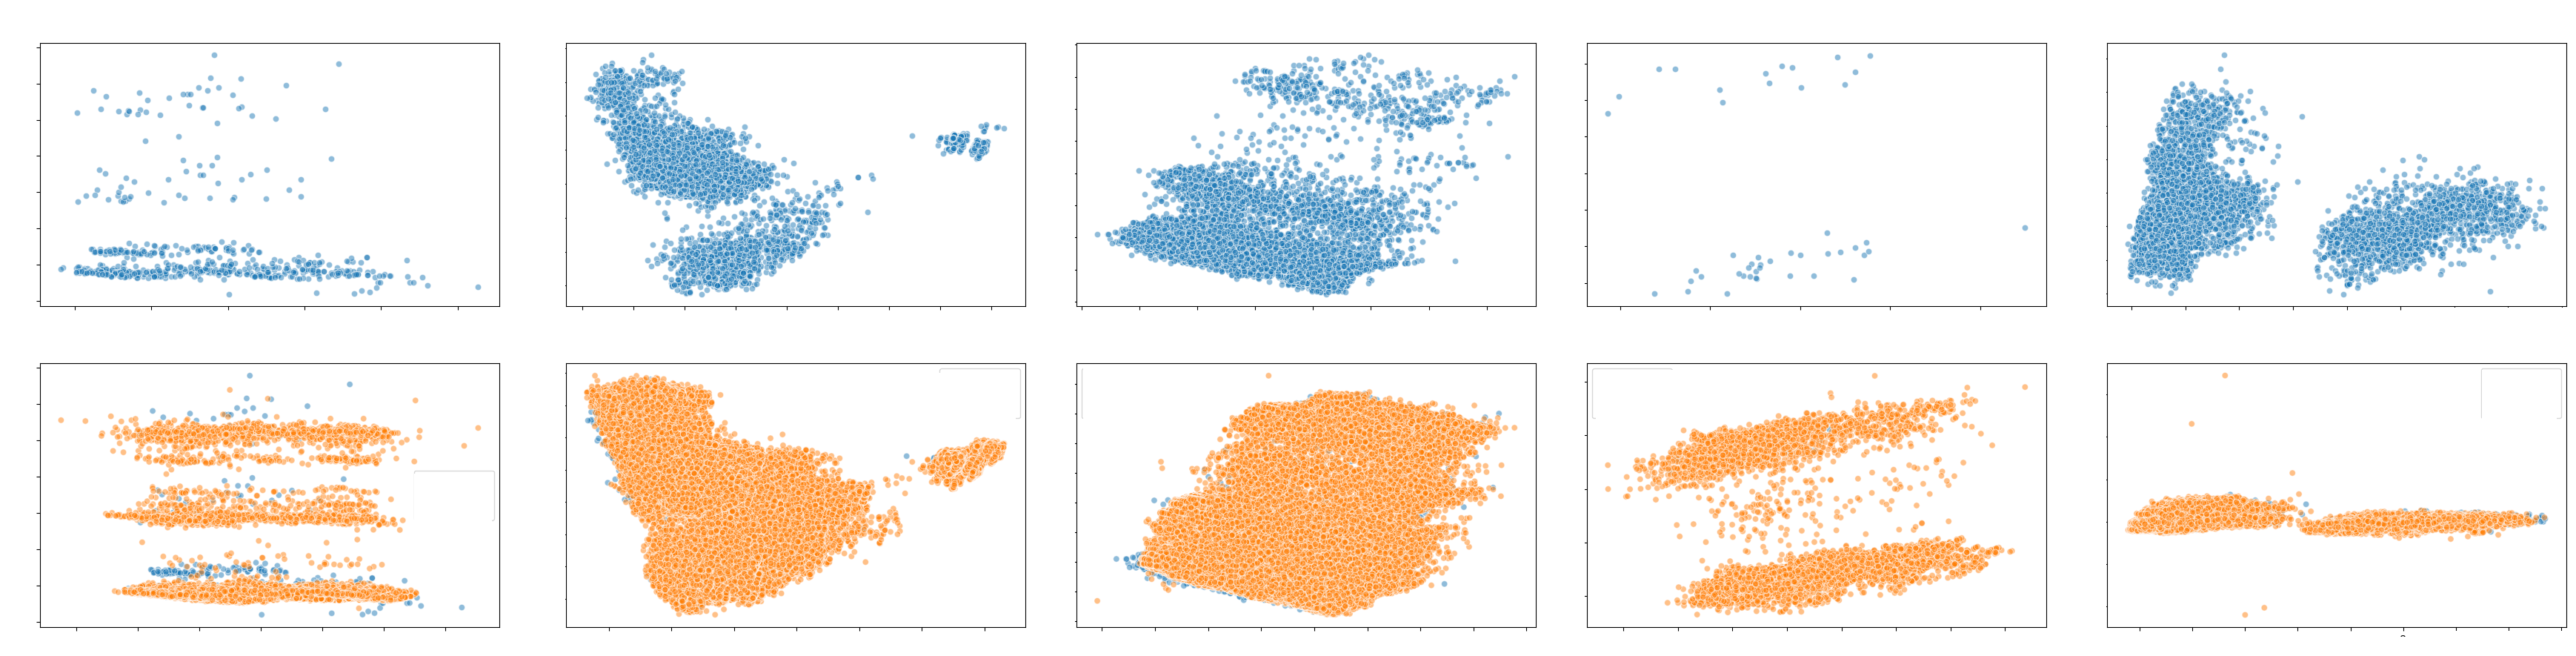
\includegraphics[width=\linewidth]{fig/ch3-pca-plot-all-features.png}
        \label{fig:pca-plot:all-features}
    \end{figure}
\end{frame}

%%

\begin{frame}{Clustering - Number of Clusters} 
    \begin{figure}
        \caption{PCA Plot for firmographics data.}
        \centering
        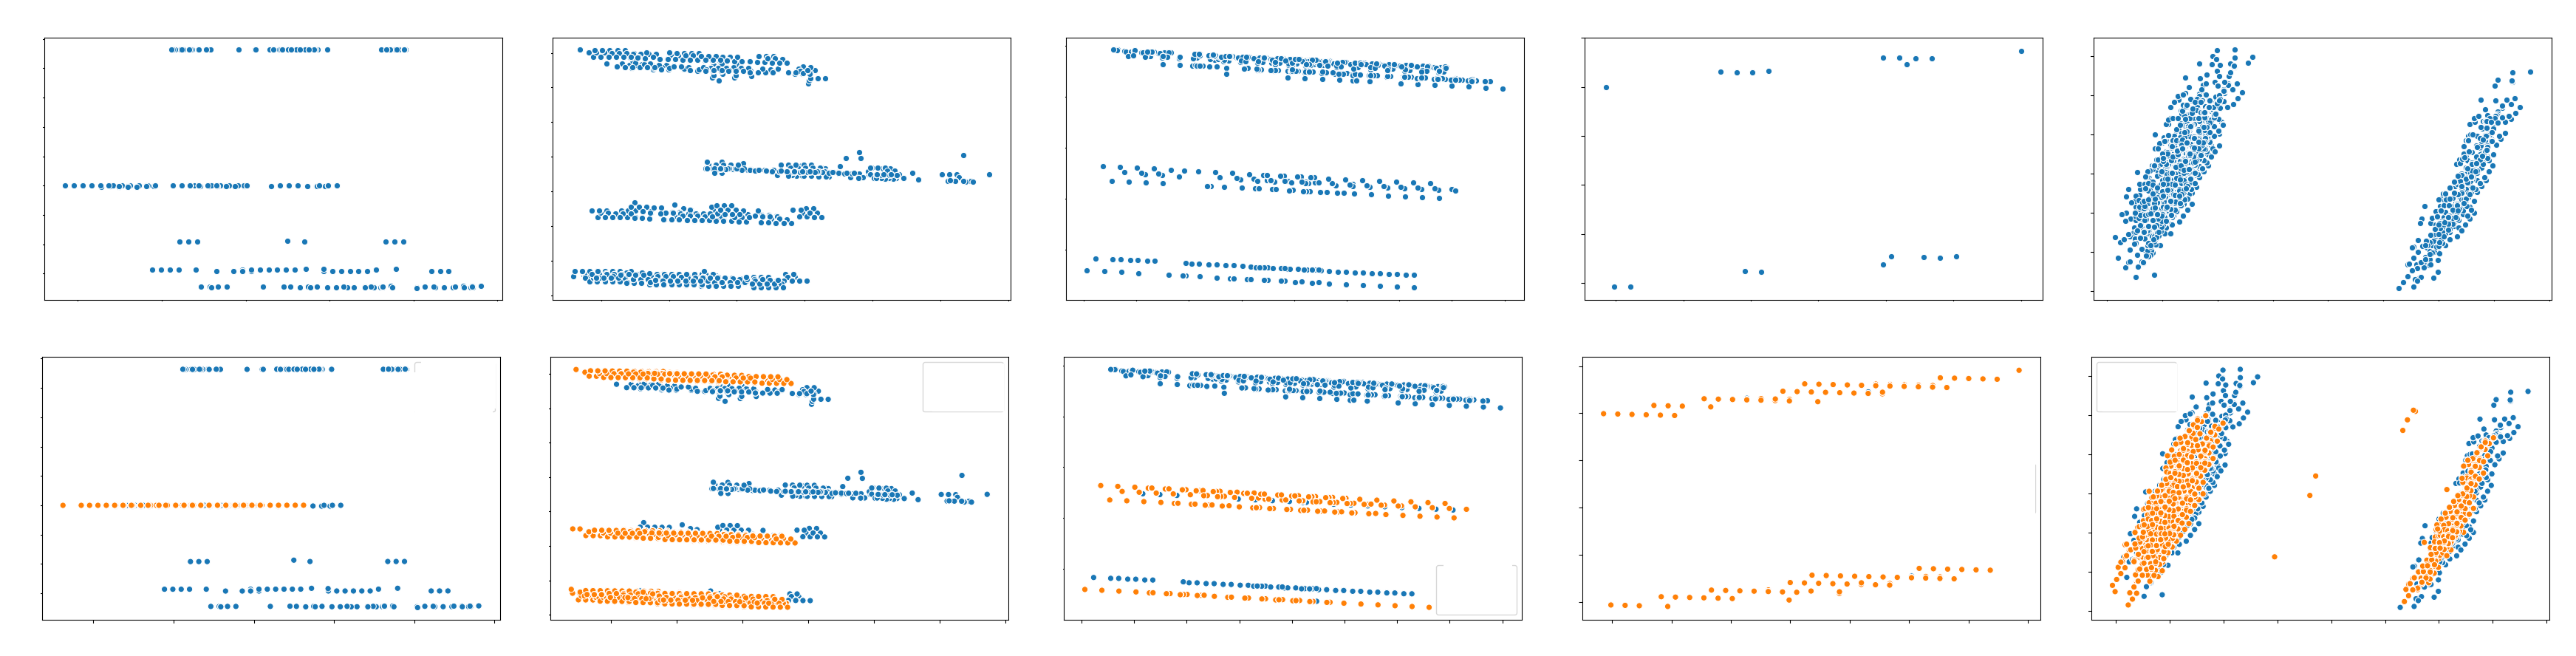
\includegraphics[width=\linewidth]{fig/ch3-pca-plot-firmographics.png}
        \label{fig:pca-plot:firmographics}
    \end{figure}
\end{frame}

%

\begin{frame}{Clustering - Algorithm} \pause
    Manual \\
    \vspace{0.5cm}
    KMeans \\  
    \vspace{0.5cm}
    Gaussian Mixture Model (GMM) \\ 
    \vspace{0.5cm}
    Bayesian Gaussian Mixture (Bayesian GM) \\
    \vspace{0.5cm}
    \only<2>{DBSCAN}\only<3->{\sout{DBSCAN}} \\
    \vspace{0.5cm}
    \only<2>{Agglomerative Clustering}\only<3->{\sout{Agglomerative Clustering}} \\
    \vspace{0.5cm}
    \only<2>{Spectral Clustering}\only<3->{\sout{Spectral Clustering}}
\end{frame}

%%

\begin{frame}{Clustering - Algorithm}
    \begin{figure}
        \centering
        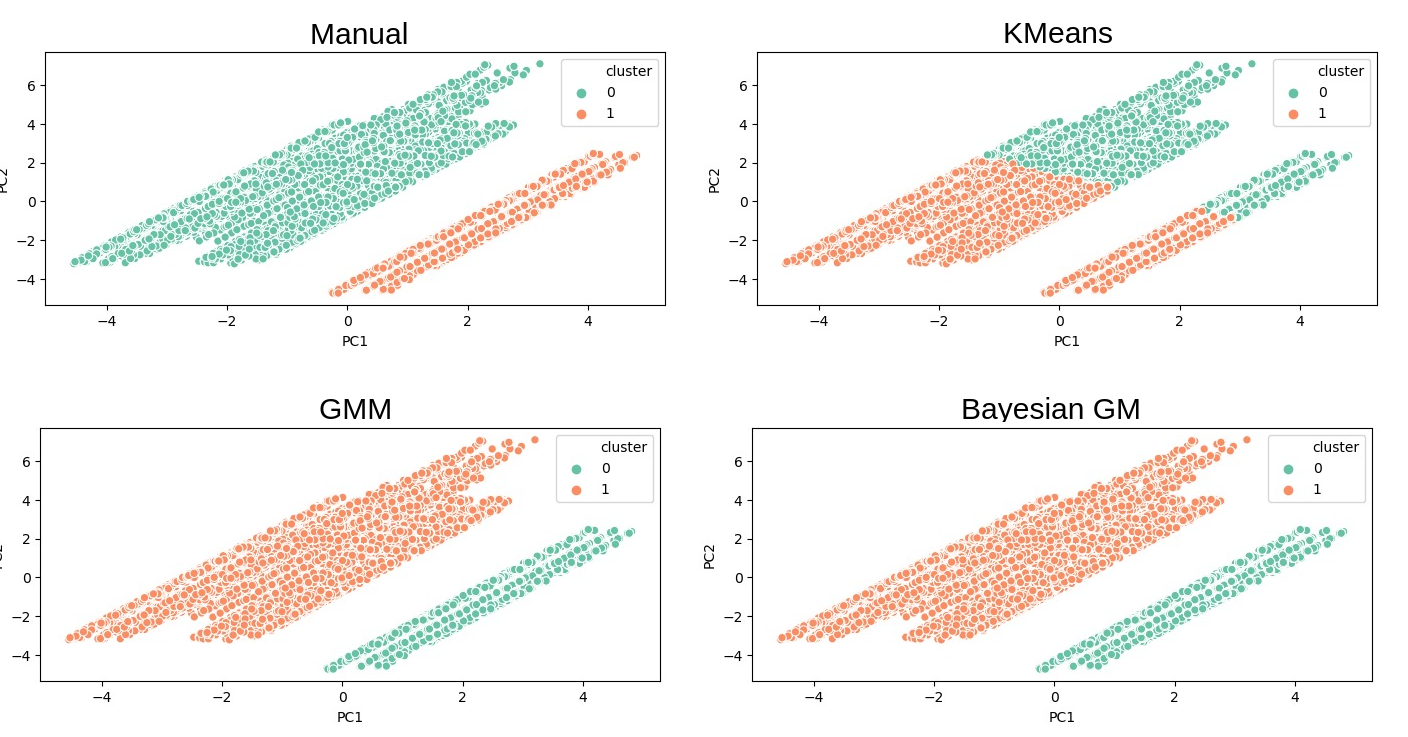
\includegraphics[width=\linewidth]{fig/ch3-cluster-algo-ex1.png}
        \label{fig:cluster-algo-ex1}
        \caption{Example clustering algorithms to study \#1.} 
    \end{figure}
\end{frame}

%%

\begin{frame}{Clustering - Algorithm}
    \begin{figure}
        \centering
        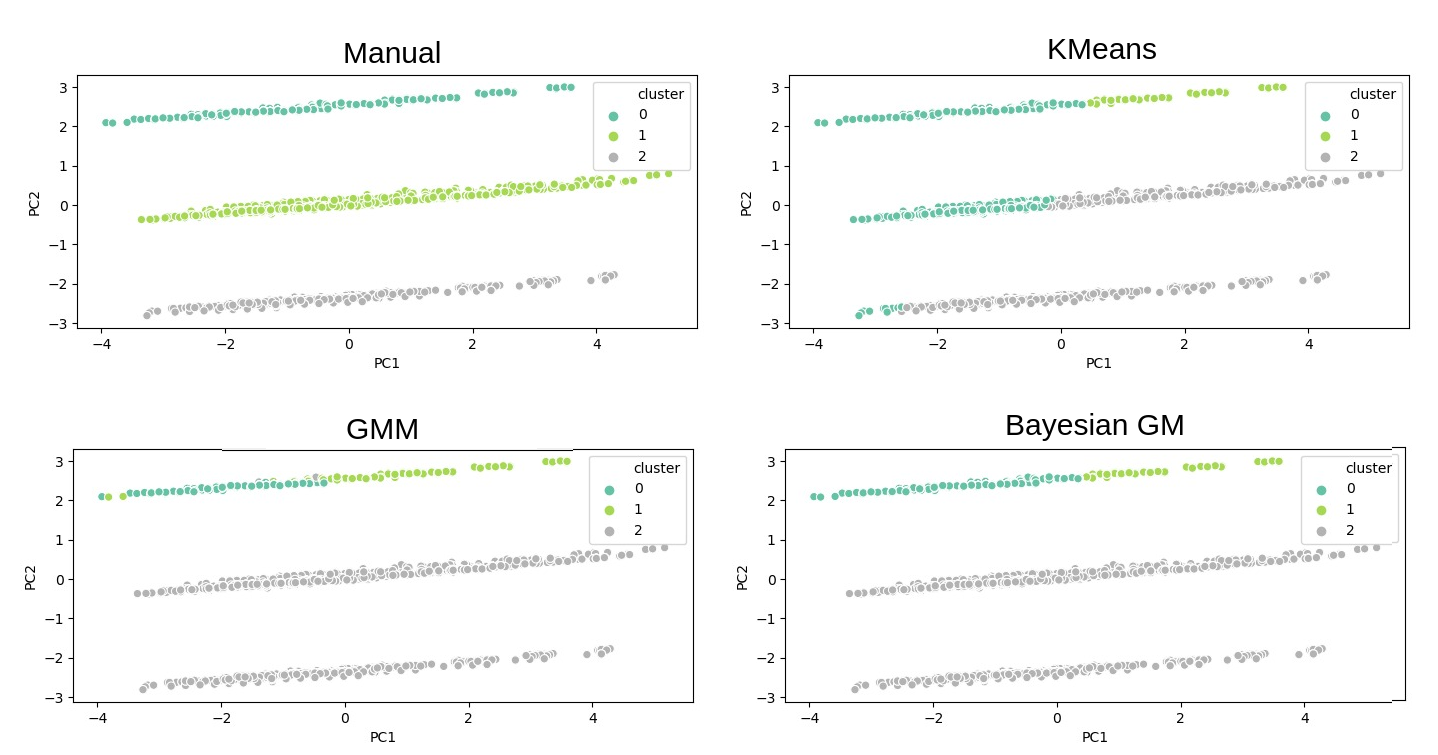
\includegraphics[width=\linewidth]{fig/ch3-cluster-algo-ex2.png}
        \label{fig:cluster-algo-ex2}
        \caption{Example clustering algorithms to study \#2.} 
    \end{figure}
\end{frame}

%%

\begin{frame}{Clustering - Algorithm}
    \begin{figure}
        \centering
        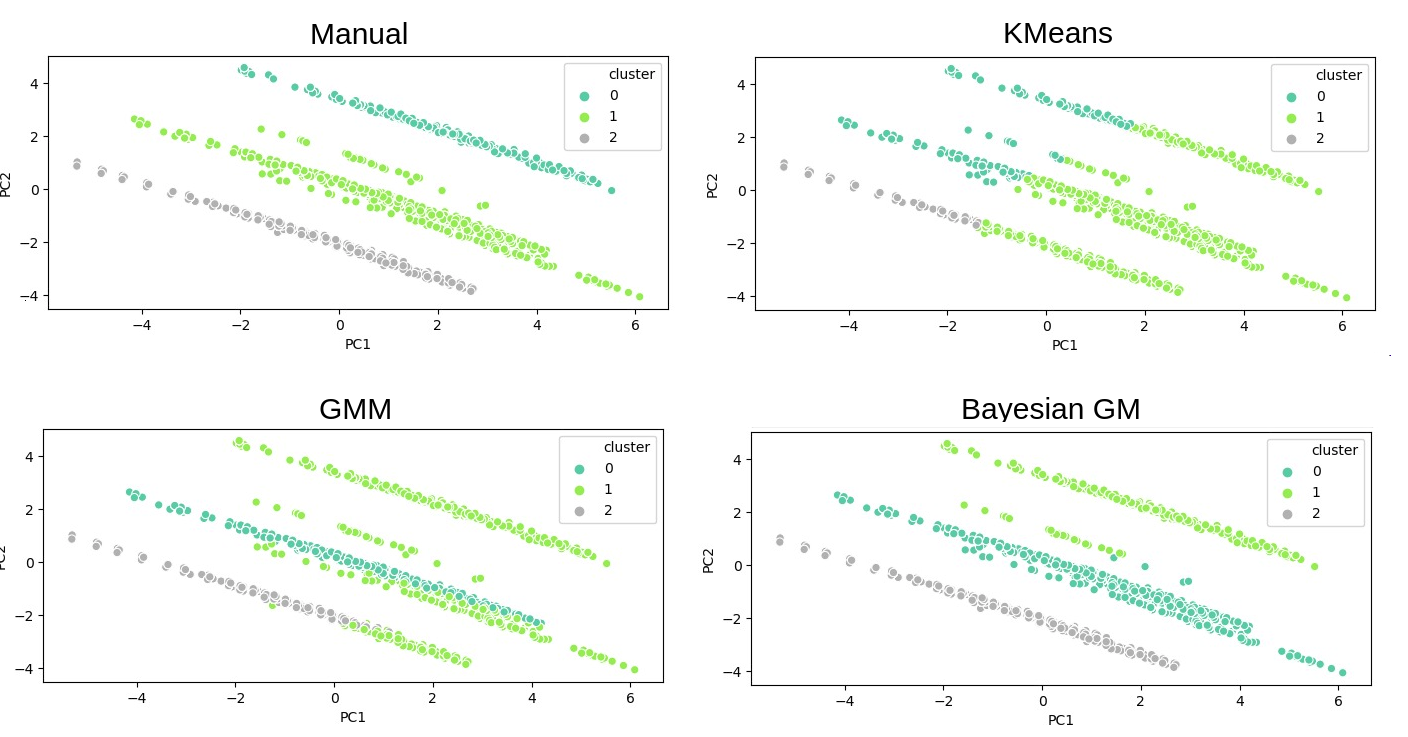
\includegraphics[width=\linewidth]{fig/ch3-cluster-algo-ex3.png}
        \label{fig:cluster-algo-ex3}
        \caption{Example clustering algorithms to study \#3.} 
    \end{figure}
\end{frame}

%%

\begin{frame}{Experiments} \pause
    Two experiments: \pause
    \begin{itemize}
        \item \fullNameExperimentI{} (\nameExperimentI{}) \pause
        \item \fullNameExperimentII{} (\nameExperimentII{})
    \end{itemize}
\end{frame}

%%

\begin{frame}{Experiments - \fullNameExperimentI{}}
    \begin{figure}
        \centering
        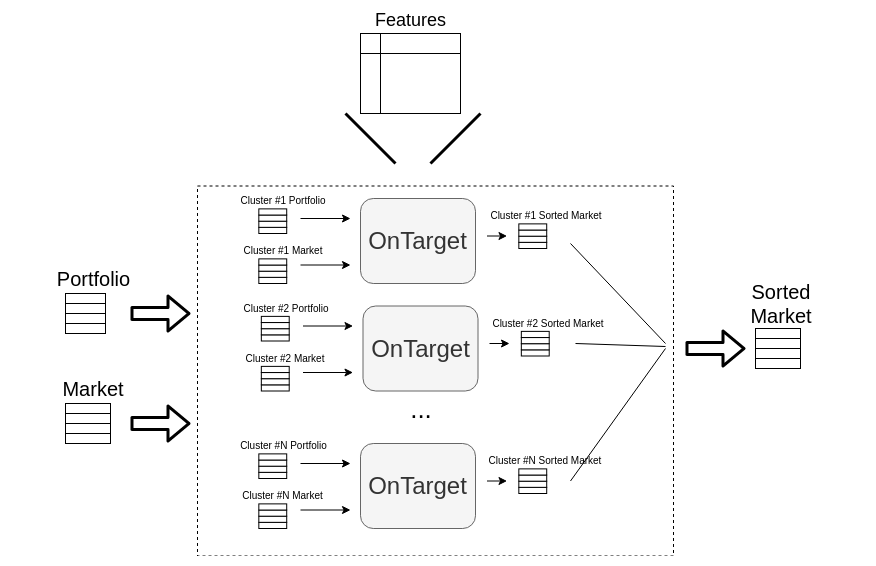
\includegraphics[width=.9\linewidth]{fig/ch3-one-run-each-cluster.png}
        \label{fig:one-run-each-cluster}
        \caption{Modifications on the OT for the experiment \nameExperimentI{}.} 
    \end{figure}
\end{frame}

%%

\begin{frame}{Experiments - \fullNameExperimentII{}}
    \begin{figure}
        \centering
        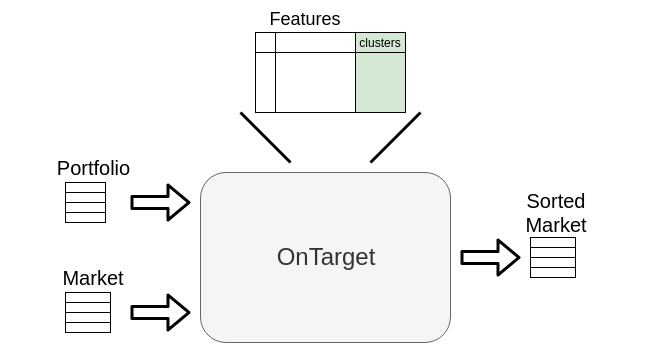
\includegraphics[width=\linewidth]{fig/ch3-clusters-as-features.png}
        \label{fig:clusters-as-features}
        \caption{Modifications on the OT for the experiment \nameExperimentII{}.} 
    \end{figure}
\end{frame}